%% The first command in your LaTeX source must be the \documentclass command.
%%%% Small single column format, used for CIE, CSUR, DTRAP, JACM, JDIQ, JEA, JERIC, JETC, PACMCGIT, TAAS, TACCESS, TACO, TALG, TALLIP (formerly TALIP), TCPS, TDSCI, TEAC, TECS, TELO, THRI, TIIS, TIOT, TISSEC, TIST, TKDD, TMIS, TOCE, TOCHI, TOCL, TOCS, TOCT, TODAES, TODS, TOIS, TOIT, TOMACS, TOMM (formerly TOMCCAP), TOMPECS, TOMS, TOPC, TOPLAS, TOPS, TOS, TOSEM, TOSN, TQC, TRETS, TSAS, TSC, TSLP, TWEB.
% \documentclass[acmsmall]{acmart}

%%%% Large single column format, used for IMWUT, JOCCH, PACMPL, POMACS, TAP, PACMHCI
% \documentclass[acmlarge,screen]{acmart}

%%%% Large double column format, used for TOG
% \documentclass[acmtog, authorversion]{acmart}

%%%% Generic manuscript mode, required for submission
%%%% and peer review
\documentclass[manuscript, anonymous, review]{acmart}
\usepackage{todonotes}
\usepackage{xcolor}
\usepackage{subfig}
\usepackage{caption}

%% Fonts used in the template cannot be substituted; margin 
%% adjustments are not allowed.
%%
%% \BibTeX command to typeset BibTeX logo in the docs
\AtBeginDocument{%
  \providecommand\BibTeX{{%
    \normalfont B\kern-0.5em{\scshape i\kern-0.25em b}\kern-0.8em\TeX}}}

%% Rights management information.  This information is sent to you
%% when you complete the rights form.  These commands have SAMPLE
%% values in them; it is your responsibility as an author to replace
%% the commands and values with those provided to you when you
%% complete the rights form.
\setcopyright{acmcopyright}
\copyrightyear{2018}
\acmYear{2018}
\acmDOI{XXXXXXX.XXXXXXX}

%% These commands are for a PROCEEDINGS abstract or paper.
\acmConference[Conference acronym 'XX]{Make sure to enter the correct conference title from your rights confirmation emai}{June 03--05,
  2018}{Woodstock, NY}


\acmBooktitle{Woodstock '18: ACM Symposium on Neural Gaze Detection, June 03--05, 2018, Woodstock, NY} 
\acmPrice{15.00}
\acmISBN{978-1-4503-XXXX-X/18/06}


%%
%% Submission ID.
%% Use this when submitting an article to a sponsored event. You'll
%% receive a unique submission ID from the organizers
%% of the event, and this ID should be used as the parameter to this command.
%%\acmSubmissionID{123-A56-BU3}

%%
%% end of the preamble, start of the body of the document source.
\begin{document}

%%
%% The "title" command has an optional parameter,
%% allowing the author to define a "short title" to be used in page headers.
\title{Empathic Smart Hybrid Buildings}

%%
%% The "author" command and its associated commands are used to define
%% the authors and their affiliations.
%% Of note is the shared affiliation of the first two authors, and the
%% "authornote" and "authornotemark" commands
%% used to denote shared contribution to the research.
\author{Shruti Rao}
\email{s.rao@uva.nl}
\orcid{1234-5678-9012}
\affiliation{
  \institution{University of Amsterdam}
  \city{Amsterdam}
  \country{The Netherlands}
}



%%
%% By default, the full list of authors will be used in the page
%% headers. Often, this list is too long, and will overlap
%% other information printed in the page headers. This command allows
%% the author to define a more concise list
%% of authors' names for this purpose.
\renewcommand{\shortauthors}{Rao et al.}

%%
%% The abstract is a short summary of the work to be presented in the
%% article.
\begin{abstract}
%   Abstracts should be about 150 words.
Given that people spend a significant amount of time within ``smart built spaces", designing spaces considering the impact that it may have on occupants’ comfort and emotions is a challenge for Human-Building Interaction (HBI).

In this position paper, we offer the view of designing smart buildings through the lens of material experiences design, whereby materials (both tangible and intangible) may impact occupants experiences of comfort and emotions.

To that end, we describe our case study and how our expected findings may aid in identification of novel, subjective human experiences (sensory, affective, interpretive and performative) with materials in hybrid spaces.

These cues may serve as a preliminary step towards designing comfort-enabling materials  and experiences in a smart, hybrid learning environment. 
\end{abstract}

%%
%% The code below is generated by the tool at http://dl.acm.org/ccs.cfm.
%% Please copy and paste the code instead of the example below.
%%

\begin{CCSXML}
<ccs2012>
   <concept>
       <concept_id>10003120</concept_id>
       <concept_desc>Human-centered computing</concept_desc>
       <concept_significance>500</concept_significance>
       </concept>
   <concept>
       <concept_id>10003120.10003123</concept_id>
       <concept_desc>Human-centered computing~Interaction design</concept_desc>
       <concept_significance>500</concept_significance>
       </concept>
 </ccs2012>
\end{CCSXML}

\ccsdesc[500]{Human-centered computing}
\ccsdesc[500]{Human-centered computing~Interaction design}

%%
%% Keywords. The author(s) should pick words that accurately describe
%% the work being presented. Separate the keywords with commas.
\keywords{affective computing, comfort, smart built environments, hybrid learning spaces, empathic design}

%% A "teaser" image appears between the author and affiliation
%% information and the body of the document, and typically spans the
%% page.
% \begin{teaserfigure}
%   \includegraphics[width=\textwidth]{sampleteaser}
%   \caption{Seattle Mariners at Spring Training, 2010.}
%   \Description{Enjoying the baseball game from the third-base
%   seats. Ichiro Suzuki preparing to bat.}
%   \label{fig:teaser}
% \end{teaserfigure}

 
%%
%% This command processes the author and affiliation and title
%% information and builds the first part of the formatted document.
\maketitle

\section{Introduction}

% Emotions in humans
Emotions serve as an implicit information communication channel between humans. Much of human communication takes place in the form of emotional exchanges that are an implicit channel for conveying information. The emotions expressed can be in the form of voice and speech, facial expressions, and behavioural patterns. These cues are recognised by humans who infer and react appropriately.

% Human-Buildings Link
In contrast to human interactions, we spend a significant amount of time inside increasingly digital buildings that creates a new dimension of relatively under-explored interaction. Information and communication technologies (ICT) and building energy management systems (BEMS) have resulted in buildings transforming from inanimate structures into interactive and communicative objects \cite{nembrini2017human}. And although buildings of the digital age can intelligently change the environmental variables (temperature, light, air quality purification) to be energy efficient and enable occupants comfort, emotion-sensing and empathic behaviour remain under-explored. 

% position
In this position paper, we consider ``smart built environments" that combine architecture with intelligent artefacts. These buildings enable for a new way of sensory perception of spaces by humans and therefore human-building interactions. We posit the need for empathic buildings that can infer occupants affective states and react appropriately to ensure occupants well being and comfort within buildings. 

% paper outline
The remainder of this paper provides a background on architecture in the digital age and the move towards human-centric buildings. We then describe our case study as a preliminary step towards understanding the perception of empathy by occupants of a smart building, and the contributions our findings can make towards empathc smart buildings.

% % comfort
% A key aspect of human experience within built environments (and by extension smart environments) is derived from the physical and emotional comfort of the occupants \cite{alavi2017comfort}. This subjective comfort which is largely as a result of qualities of the built environment can play a role in impacting the occupants awareness and behaviour within that environment.  



\section{Background}
% HBI
Human-building interaction (HBI) is a burgeoning area of research that focuses on capturing, understanding and enhancing human interactions and experiences both with and within ``smart built environments" \cite{alavi2016future}. The primary goal of HBI being a framework that can be used to understand, compare, and converge research efforts from the fields of HCI, design, and architecture in envisioning and shaping the future of living spaces and all that they encompass \cite{nembrini2017human, alavi2018artifacts}. 

% % Comfort and Affect in Built Environment
% The concept of comfort is central to occupants within built environments. Comfort is understood as occupants' physiological and affective (emotional) responses to the built environment \cite{alavi2017comfort}. HBI especially examines the relationship between occupant comfort and four physical characteristics of the indoor environment - temperature, air, light, and sound \cite{hawkes2007environmental, bluyssen2009indoor}. 

% Examples of work in buildings catering to human needs
In this context, there are several works that try to develop human-centric and responsible buildings. Smart building facades for example are being developed that adapt to the external environment and react in an energy efficient manner \cite{ahmed2015development}. There are also several works that look at providing comfort to users using responsive materials that react to temperature, light, humidity and air quality \cite{fragkia2020exergy, holstov2015hygromorphic, kroner1997intelligent}. These include designing ``optimally informative" systems such as temperature calendars, air quality forecasts, noise level indicators, and wearables that appropriately inform occupants of their environment and also allow them to engage with comfort parameters to certain degrees  \cite{costanza2016bit, milenkovic2013improving, kim2020designing}. Other works focus on a ``gamified" approach to engage users with their environment and activities in a socially inclusive manner \cite{mathur2015tiny, kwallek1997impact, zhong2022augmenting}. 

% Our perspective
Therefore, much of the work towards developing human-centric buildings focus on changing the environmental variables that may in turn impact the occupants experiences. Instead, in this position paper we wish to reconsider the design of human-centric buildings through the perspective of occupant emotions ie. buildings that respond to human emotions.


\section{Empathic Technologies for Shaping Human-Building Interactions}

% Why empathic buildings
A significant consequence of smart buildings is that occupants find themselves physically immersed within an interactive object, and therefore experience interactions in a multi-sensory manner \cite{nembrini2017human}. Understanding the exact nature of such interactions, and shaping them to positively impact humans is an important aspect of HCI.   

Providing for varied and subjective experiences to occupants within a hybrid space that is used by different people with varying usage goals is a challenge. 

Empathic buildings that understand their occupants emotions can make use of ubiquitous tangible and intangible artifacts to infer occupant emotions and shape the ways in which occupants experience emotions in buildings.

% Moreover, material
% experiences can play a more ubiquitous role in fostering occupants' interactions with non-digital elements of the building through digital means - a key concern in HBI \cite{nembrini2017human}. 

\subsection{A Digital Building of the Present}
\label{subsec:building}
Our motivation to call for empathic buildings comes from occupying and experiencing one such digital building that houses students, researchers, entrepreneurs, and businesses.

The building labelled as an ``intelligent hub" was designed to be empathic from an architectural standpoint, with a vision to be sustainable, circular and flexible, healthy, and inspiring \footnote{https://lab42.uva.nl/}. The building is designed to be more "human-centric" in the sense that spaces in the building are designed to elicit or evoke certain human emotions and sentiments. To that end, different artifacts in the interior and exterior have been designed using a variety of materials and design features. The building aims to encourage openness in the lower floors - a glass atrium is used to convey the feeling of transparency to occupants who can view all ongoing activities of the building. \todo{photo of robotics lab} A combination of colourful plinth, and display of digital artifacts are used to make occupants feel curious and stimulate collaboration. Quietness and concentration in the upper zones are indicated by recycled felt fashioned into panels and inner walls to promote acoustics. A combination of intelligent sensors throughout the building control light, temperature, and air quality to provide for comfort based on the number of occupants, and external and indoor environmental conditions.

\begin{figure}[htbp]
\centering
\subfloat[Privacy enabling curtains in a high concentration zone\label{fig:curtain}]{\includegraphics[width=0.2\textwidth]{images/privacy-curtains.jpg}}\hfill
\subfloat[Sheer fabric of the curtains questions the privacy-providing aspect.\label{fig:curtain-sheer}] {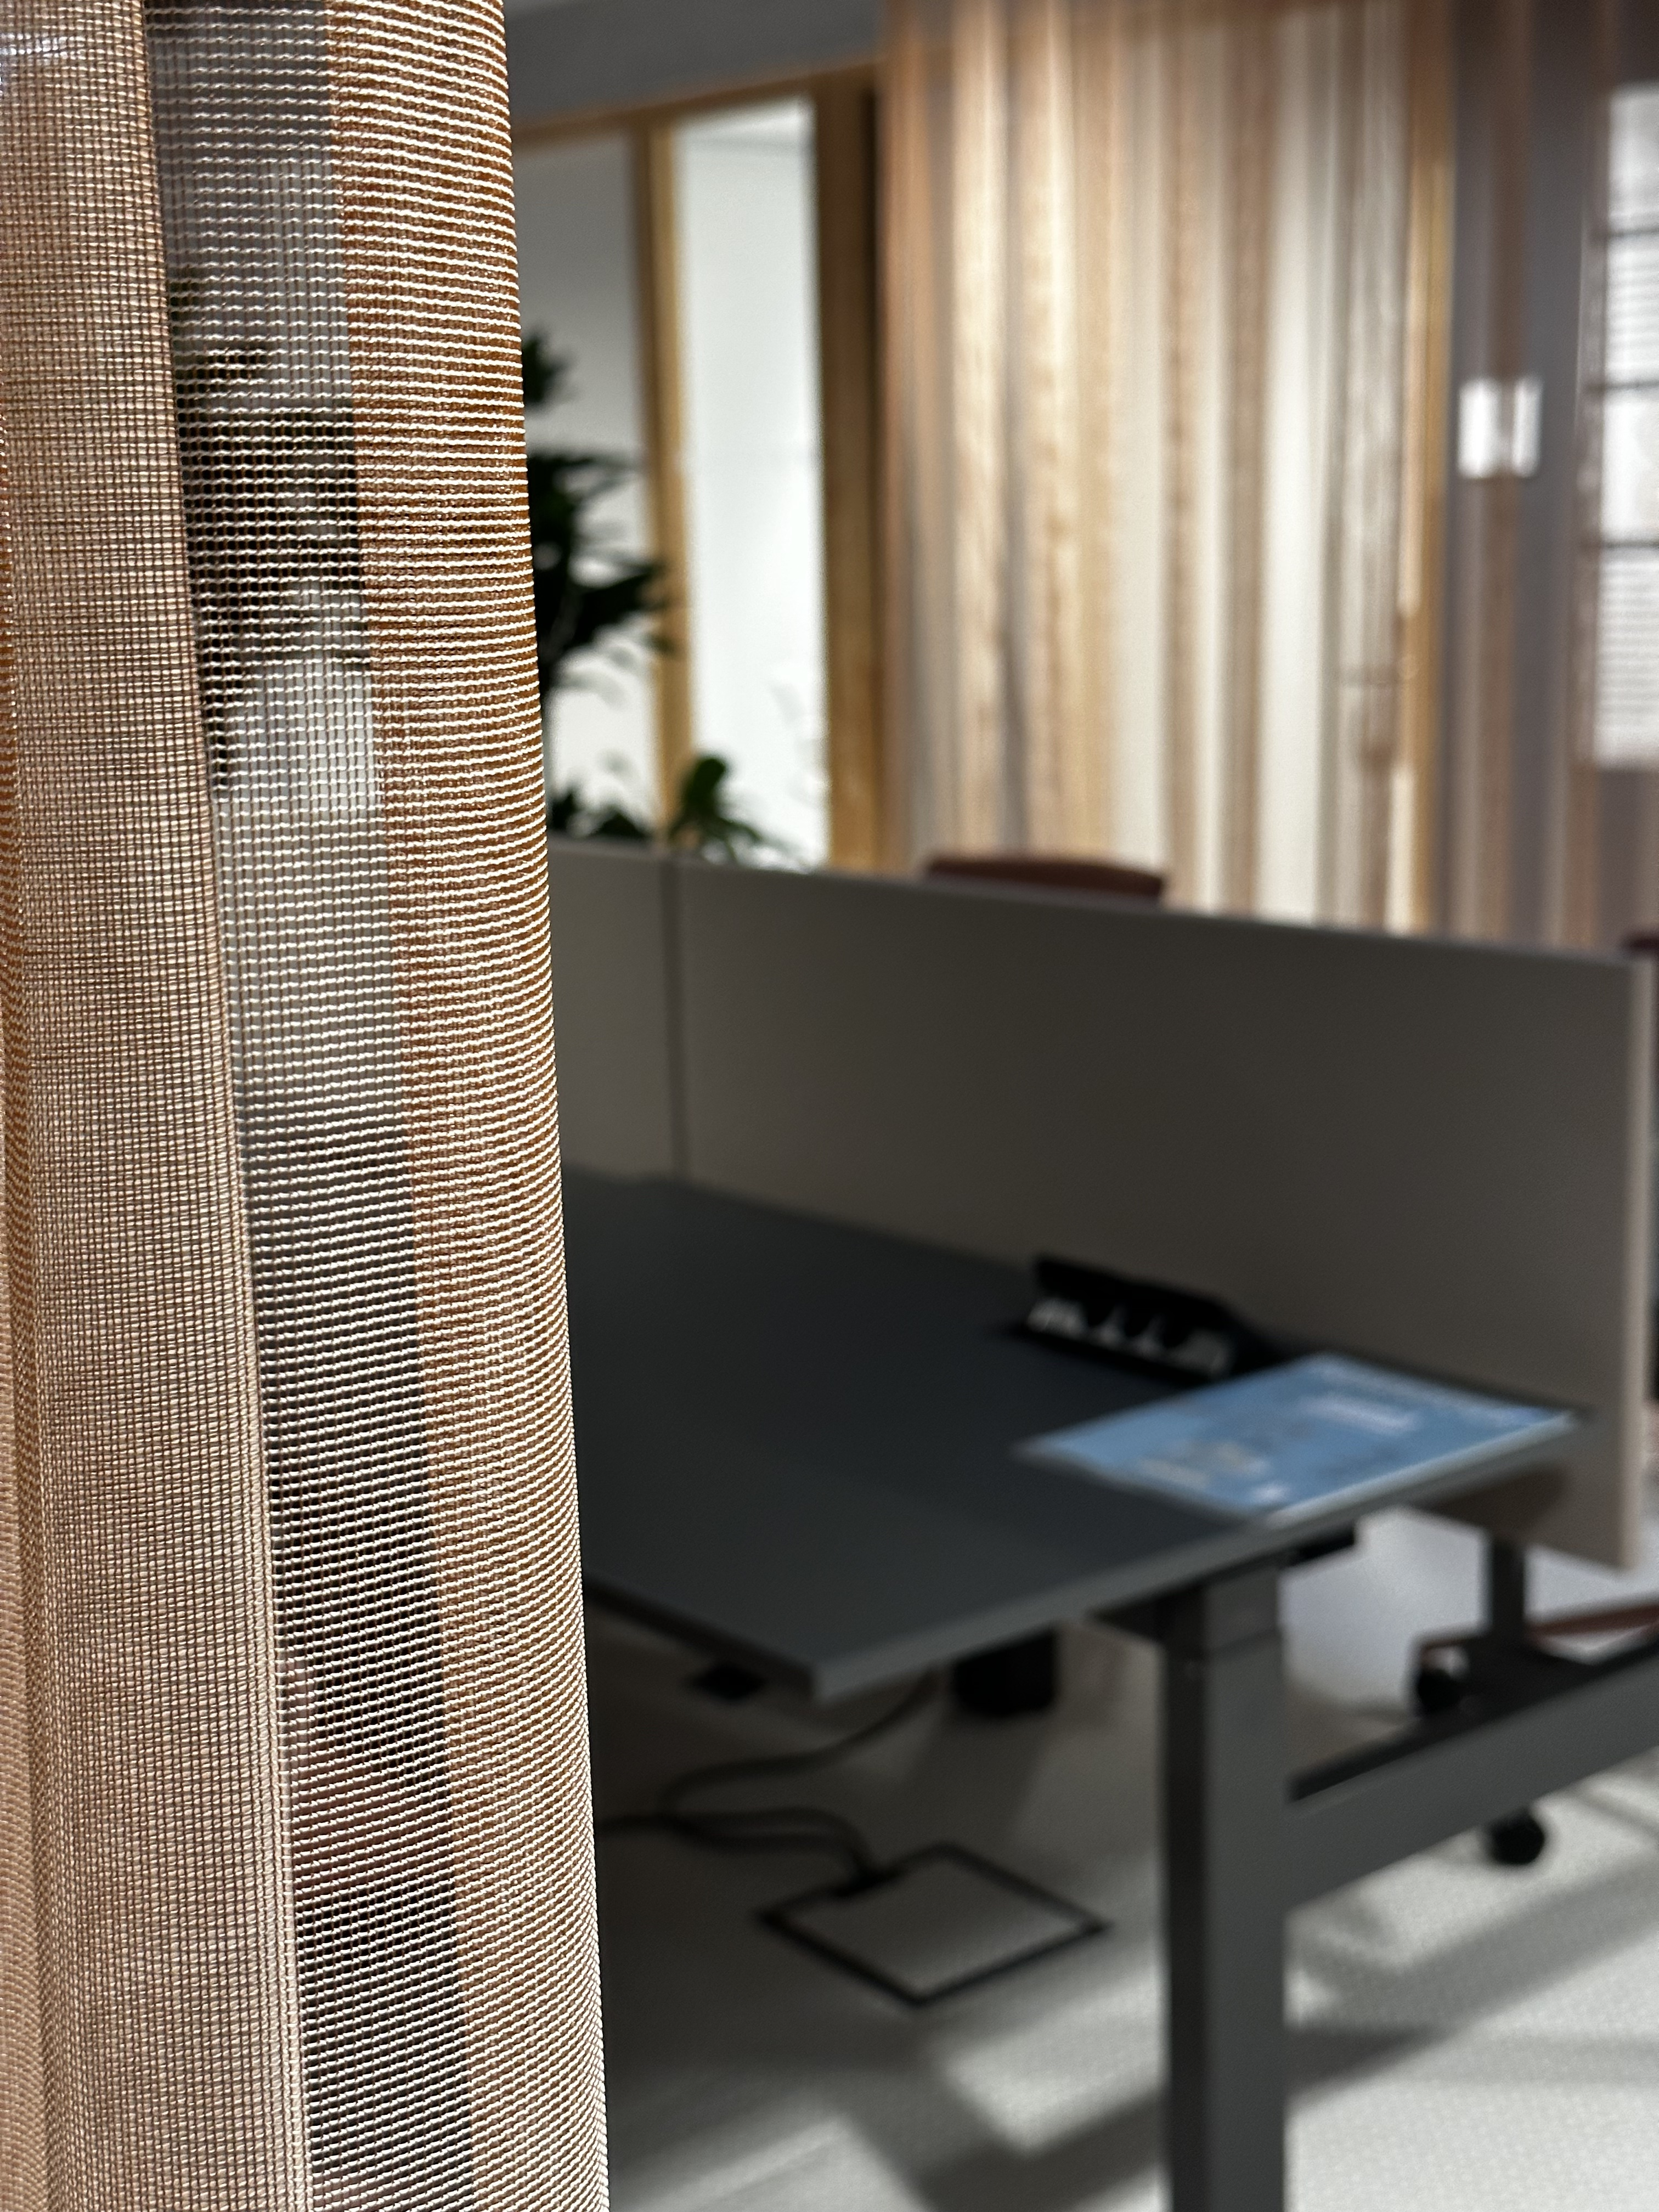
\includegraphics[width=0.2\textwidth]{images/privacy-curtains-fabric.jpg}}\hfill
\subfloat[The building staircase designed to encourage users to take the stairs.\label{fig:staircase}]{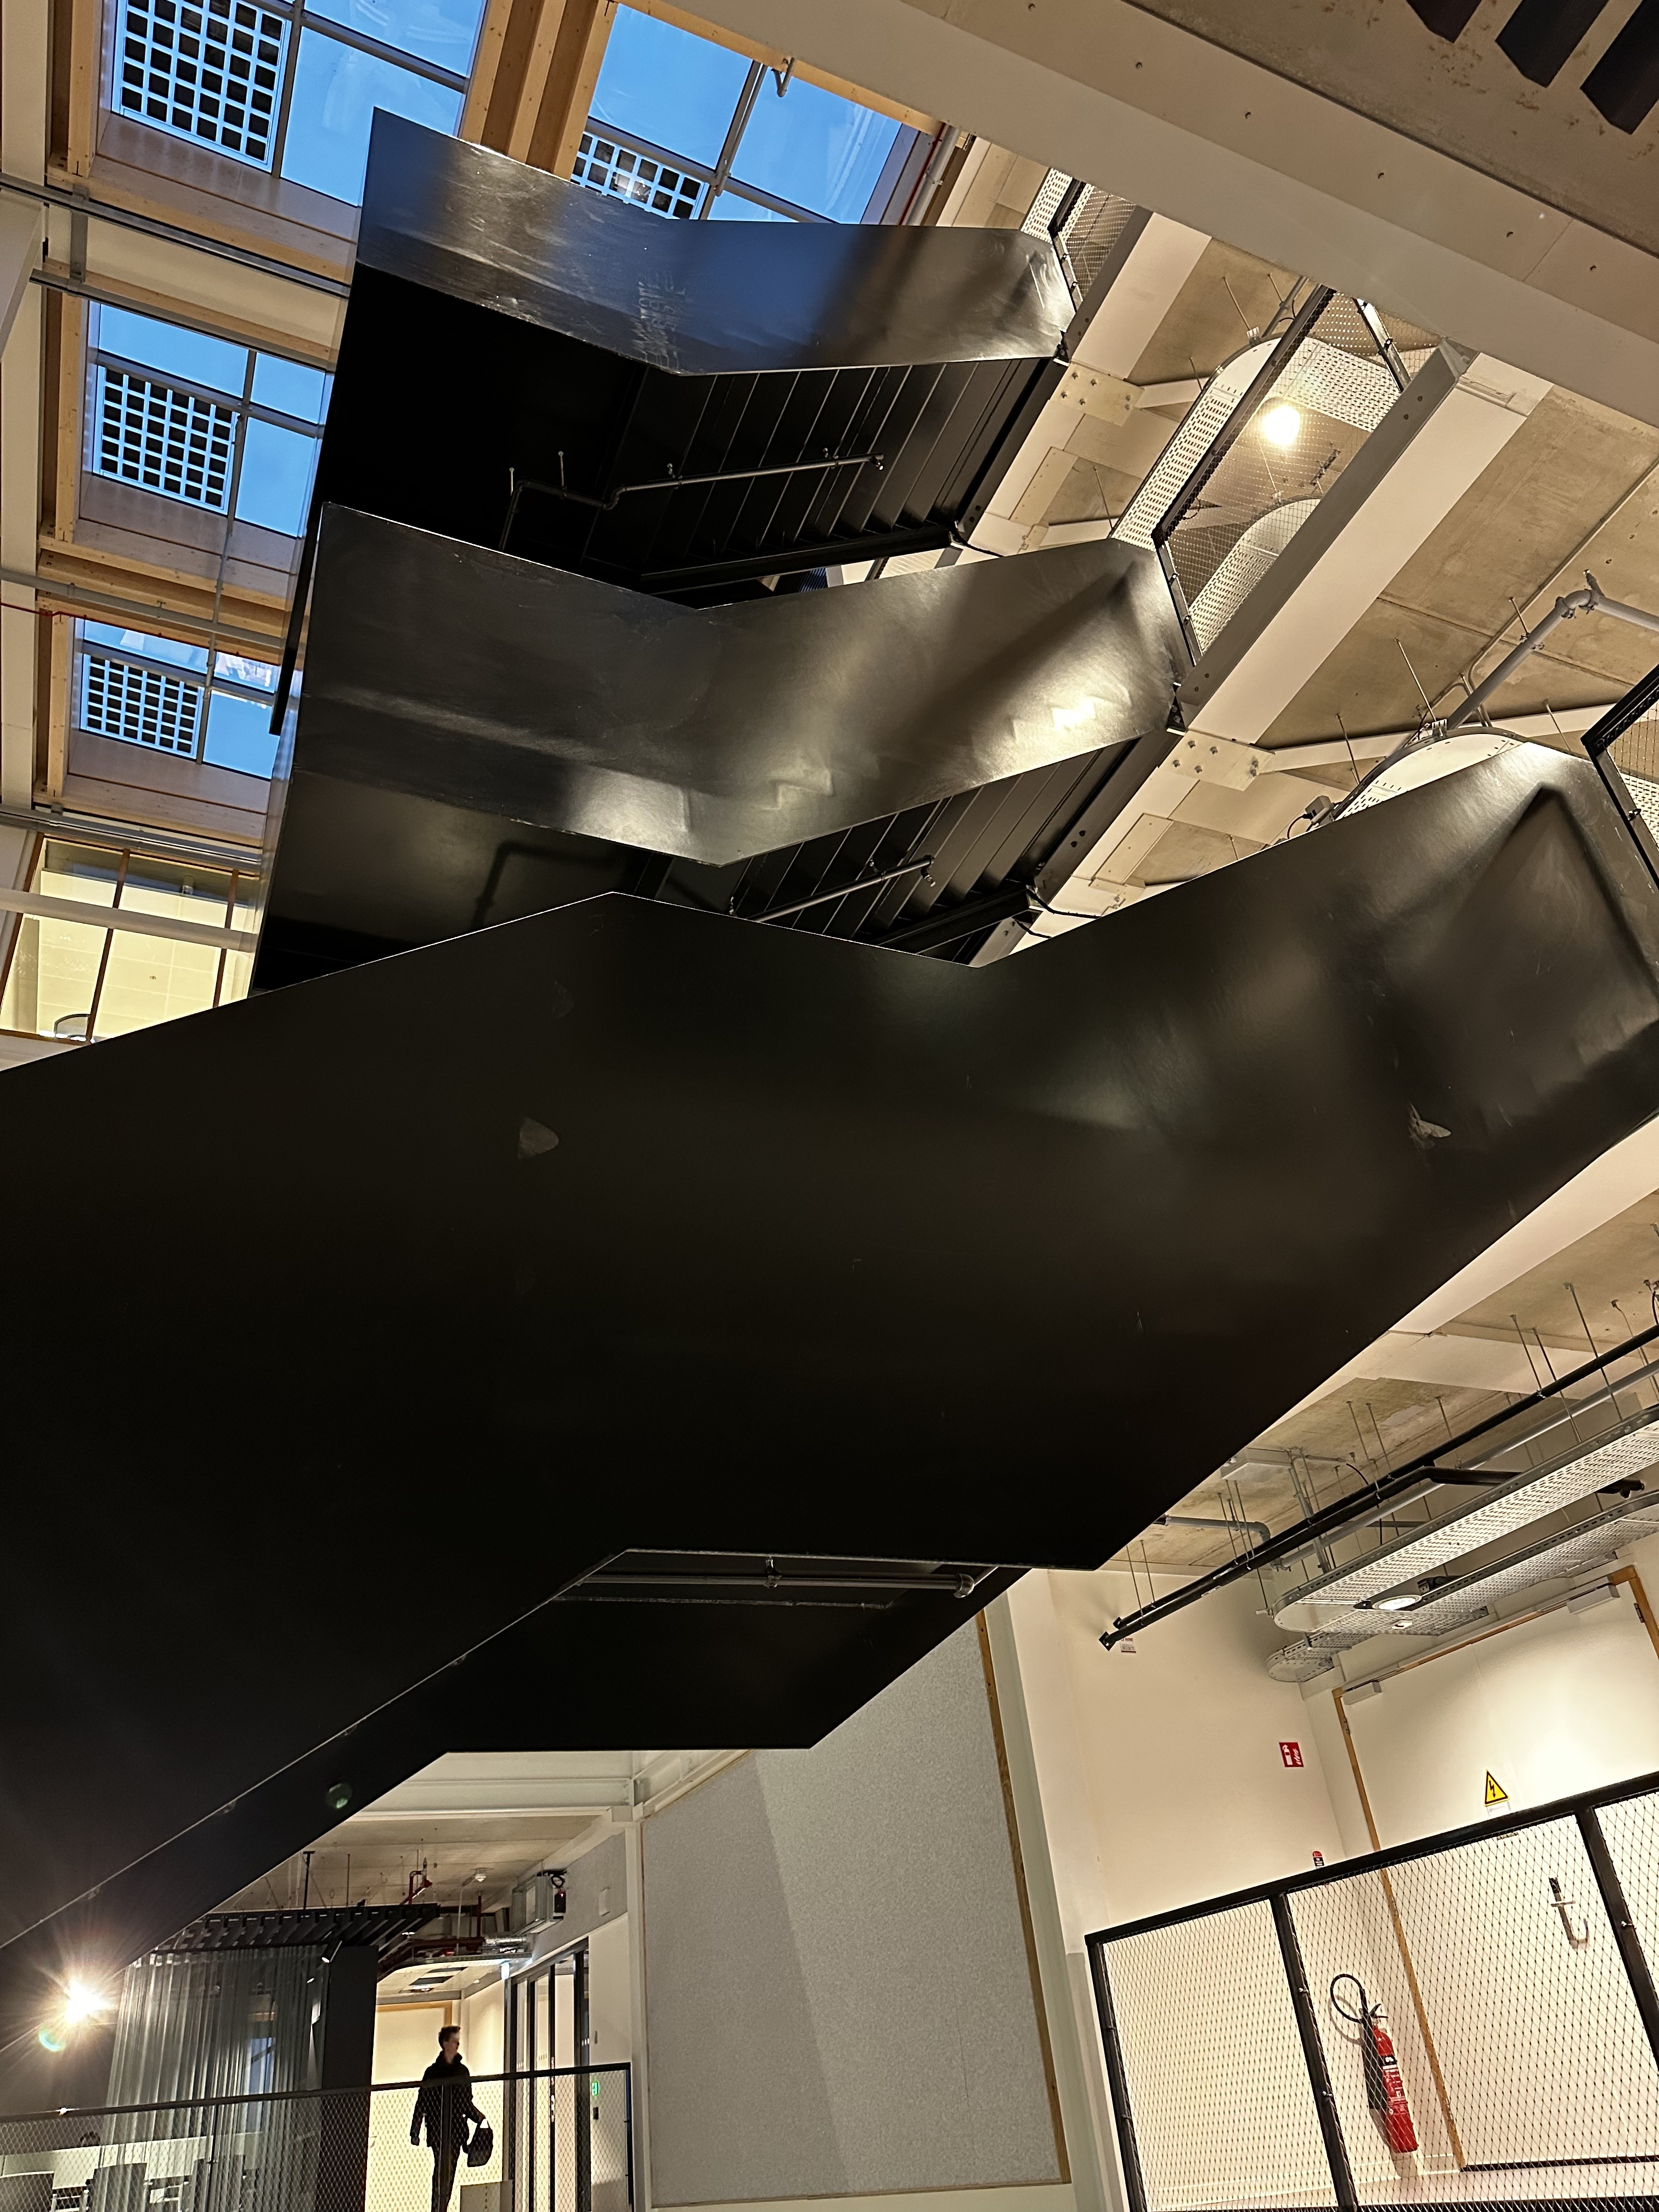
\includegraphics[width=0.2\textwidth]{images/stairs.jpg}}\hfill
\subfloat[Wrought iron railings and smooth black surfaces \label{fig:staircase-railing}]{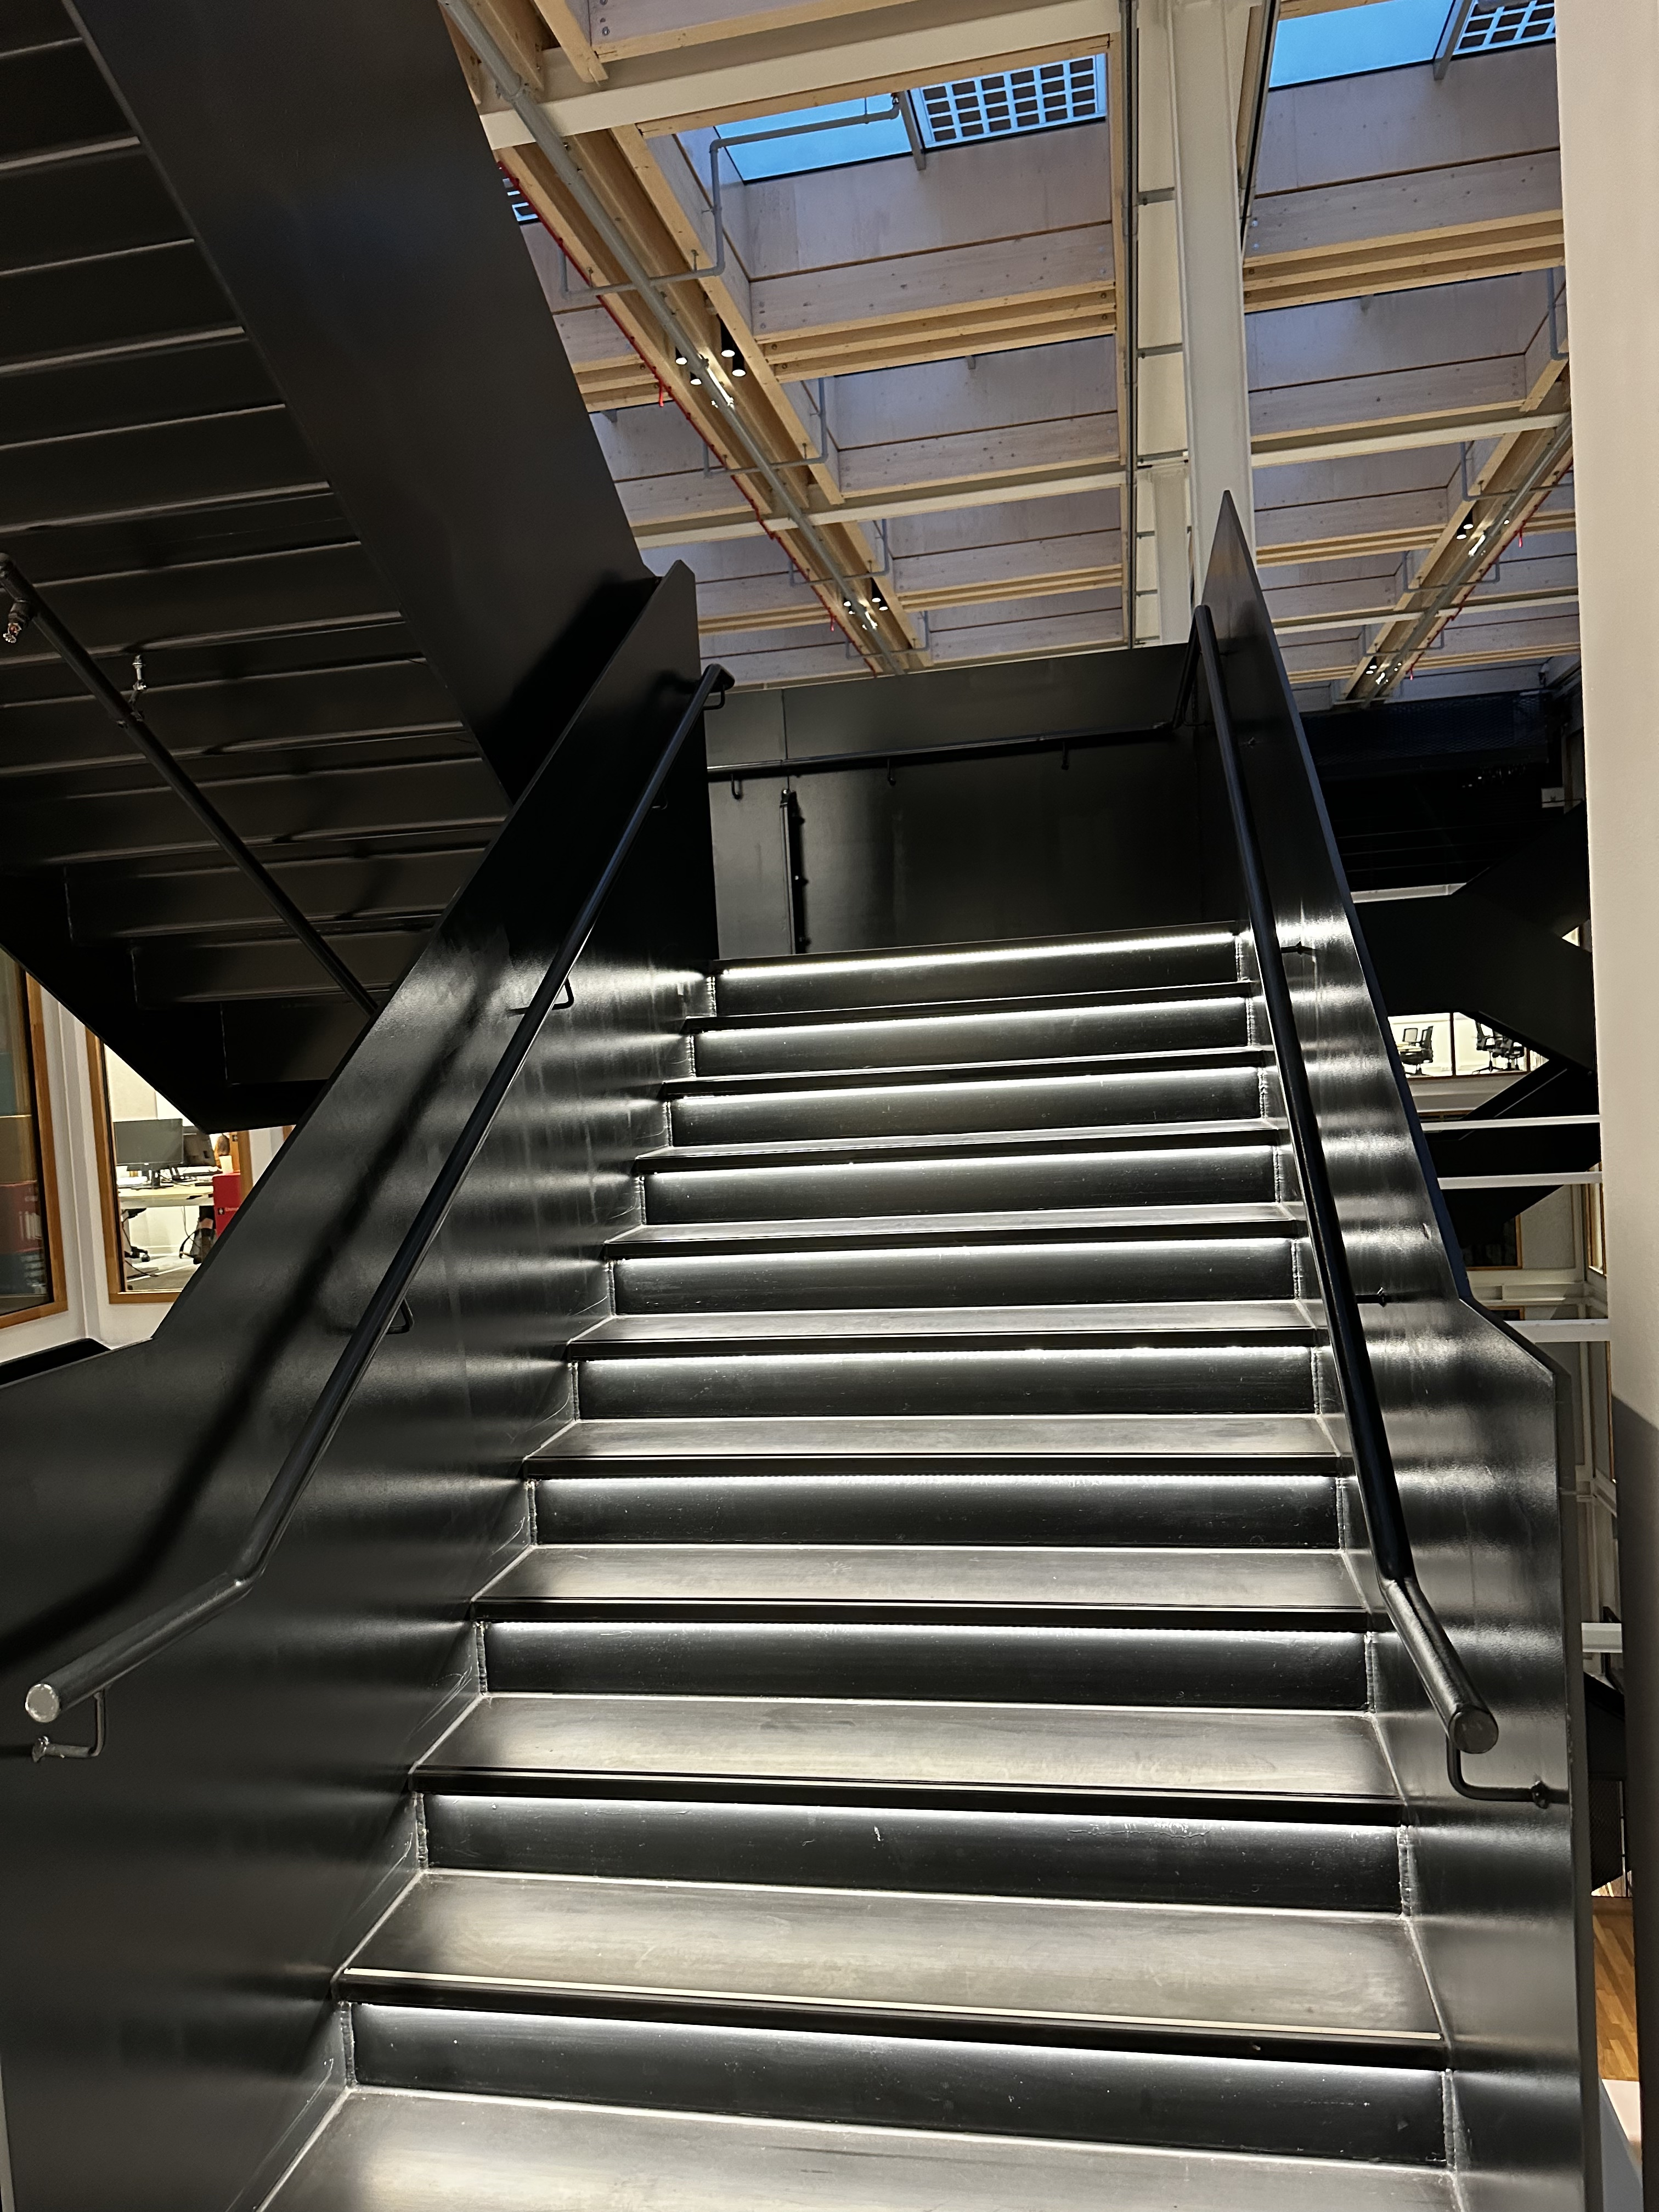
\includegraphics[width=0.2\textwidth]
{images/stairs-closeup.jpg}}
\subfloat[A large screen upon entering the building that serves as a means for communication \label{fig:screen}]{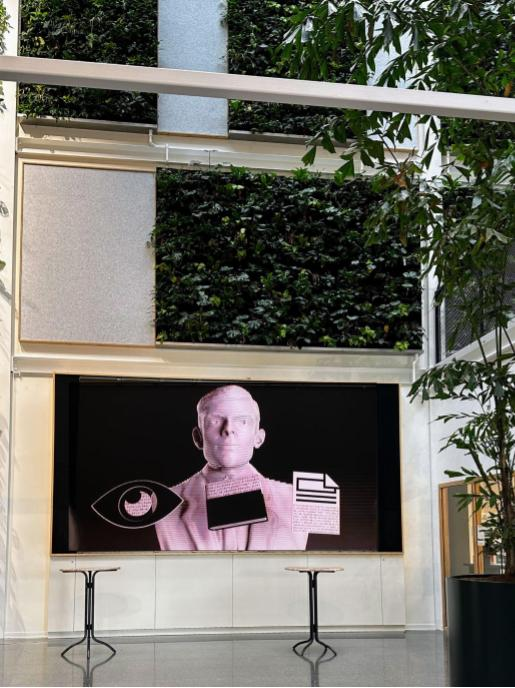
\includegraphics[width=0.2\textwidth]
{images/screen.jpg}}
\caption{Materials in a smart building that raise questions about its nature and the type of experience it provides to the buildings occupants.} \label{fig:lab42-examples}
\end{figure}

Figure \ref{fig:lab42-examples} shows three tangible artifacts in the building designed to be empathic from an architectural standpoint, but raise questions about the nature of their role in interacting with the building occupants. We speculate on the shortcomings of these artifacts and suggest how intelligent  alternatives could be employed towards truly empathic buildings.

\subsubsection*{The Privacy Curtains}
Figures \ref{fig:curtain} and \ref{fig:curtain-sheer} show curtains around certain work spaces in the middle of high-traffic corridors. The curtains serve as a means of providing a sense of privacy and recluse amidst the open and public spaces. However, the sheer material instils a feeling of transparency and therefore, the clash between the concept of privacy and a sheer curtain creates a feeling of confusion and frustration regarding its purpose. Instead, we propose that the curtains could be made  more empathic by intelligently transforming from sheer to fully opaque by in-situ inferring occupants privacy needs (for eg., sensing anxiety).  

\subsubsection*{An Encouraging Staircase}
The building promotes its staircase in Figures \ref{fig:staircase} and \ref{fig:staircase-railing} as being designed to inspire people to climb stairs rather than use a lift. However, cold and textured wrought iron railings discourages one from using it. The black, oversized, and floating structure floating, casts a foreboding  shadow on the onlooker  and the brutalist design evokes a feeling of awe - something to observe, rather than use. We find that the staircase often fails to create a feeling of encouragement and push towards using it. Alternatively, a gamified and anthropomorphised staircase that incorporates interactive materials that respond to users activities may be more suited to simulate feelings of activity. 

\subsubsection*{The Digital Interface to the Building}
\todo[]{Try to add images of interface in use}
A large screen in the building foyer accompanied by an interactive interface allows users to explore and learn different things about the building. The interface is an interactive tablet that can be accessed by clicking and moving information around. The screen presents itself a digital building attempting to be transparent and communicate with its occupants. This placement triggers intrigue in learning more about the building. However, limited information displayed prevents the device from becoming part of an occupant's daily practice (such as checking one's phone every morning). A conversational user interface (CUI) may be able to on the other hand serve a medium between the non-digital aspects of the building through a digital means. 

% Our proposed case study
\subsection{Our Proposed Case Study} 
We wish to identify artifacts or spaces in buildings where architectural features of empathy design fall short and so could benefit from a more digital design. Towards developing such an empathic architecture that can infer occupant emotions, we are undertaking a preliminary case study in the aforementioned building. We aim to identify occupants' novel and subjective experiences that arise from interactions within the smart building. We are particularly interested in understanding experiences of occupant comfort (based on the indoor environmental) and emotions \cite{alavi2017comfort} which is key in built environments.  We wish to thereafter identify specific influential factors (tangible and intangible) that determine the overall sense of comfort and emotions in smart buildings spaces. The case study comprises two phases: (a) emotion and comfort label collection, and (b) building walk. First, we will conduct a short survey to obtain a large number of occupant emotion and comfort information based on different spaces in the building. Next, a building walk will be organised to obtain an in-depth understanding of occupants' perceptions - mental, emotional and physical towards different spaces in the building.

During the walk, researchers will engage participants in conversations about each space, and conversations will form around what users expect of an empathic building of the future. Questions will investigate different experiential levels (sensory, interpretive, affective and performative) and will include asking about impressions of the space, usage of space \textit{(How would you use this space? Why do you use this space? What kind of tasks would you perform in this space?)}, emotions in the space \textit{(What emotions do you associate with this space?)}, comfort \textit{(Is this space comfortable? Is there sufficient light, warmth, ventilation?)}, shortcomings and scope for improvement. Data collected from both phases will be analysed using thematic analysis, and lexical analysis \cite{braun2006using, xue2020mood}. 

\subsection{Privacy Considerations}
\todo{}

\subsection{Expected Contributions}
Through our case study, we aim to identify specific artifacts both tangible and intangible, and the properties of these artifacts that impact building occupants' emotions. Additionally, we expect to gain an understanding of the lived-in bodily comfort and emotional experiences within smart learning spaces from an affective, and interpretive perspective \cite{giaccardi2015foundations}. Through our work, we aim to identify design spaces and artifacts that fail to fulfil an empathic role for the occupants. Our work is a preliminary step towards design and development of spaces that can understand and assist in the emotional and comfort needs of occupants help  to create experiences that occupants might find lacking in smart buildings (for eg., sense of autonomy and control in an automated building) \cite{moreno2014user}, or enhance certain other experiences (for eg., feeling of groundedness and familiarity in a space used by many) \cite{rehman2022personalisedcomfort}. We envision that our work forms the qualitative step twoards understanding users expectations from an empathic building and therby design for solutions that in-situ infer occupants (negative) affective states, and attempts to alter it through means of emapthic responses. 







\section{Conclusion}
The increased complexity of built environments in recent years can be attributed to a growing expectation for buildings to adapt to changing socio-environmental parameters. Given the inevitable growth of smart built environments, in this position paper we suggest that buildings be designed to be empathic to its occupants by understanding and responding to their affective states. We put forth consideration of empathic spaces in smart buildings. We discuss how artifacts (tangible and intangible) in smart buildings can be examined, understood and thereby designed for occupants' subjective needs and experiences. To that end, we highlight a case study that we will undertake to identify understand the impact of one such smart building and it's artifacts (tangible and intangible) on its'  occupants, and therefore needs rethinking and redesign such that they may serve as catalysts for improved human experiences of comfort and wellbeing. 


\bibliographystyle{ACM-Reference-Format}
\bibliography{affective-comfort}

\end{document}
